\documentclass{article}
\usepackage{amsmath}
\usepackage{listings}
\usepackage{xcolor}
\usepackage{graphicx}
\usepackage{geometry}
\usepackage{hyperref}
\usepackage{tikz}
\usetikzlibrary{trees, positioning}
\geometry{margin=1in}

\title{Binary Search Trees}
\author{}
\date{}

\definecolor{codegray}{rgb}{0.5,0.5,0.5}
\definecolor{backcolour}{rgb}{0.95,0.95,0.92}

\lstdefinestyle{cppstyle}{
  backgroundcolor=\color{backcolour},
  commentstyle=\color{codegray},
  keywordstyle=\color{blue},
  numberstyle=\tiny\color{codegray},
  stringstyle=\color{red},
  basicstyle=\ttfamily\footnotesize,
  breakatwhitespace=false,
  breaklines=true,
  captionpos=b,
  keepspaces=true,
  numbers=none,
  numbersep=5pt,
  showspaces=false,
  showstringspaces=false,
  showtabs=false,
  tabsize=2,
  language=C++
}

\begin{document}

\maketitle

A \textbf{Binary Search Tree (BST)} is a binary tree where each node contains a key such that:
\[
\texttt{left subtree keys} < \texttt{node key} < \texttt{right subtree keys}
\]
This ordering enables efficient searching, insertion, and deletion operations.

\section{Example BST Structure}

\begin{center}
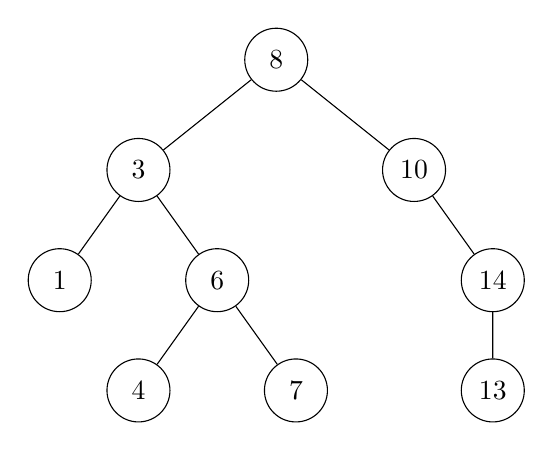
\begin{tikzpicture}[
  every node/.style={circle, draw, minimum size=0.8cm},
  level distance=1.4cm,
  level 1/.style={sibling distance=3.5cm},
  level 2/.style={sibling distance=2cm}
]
\node {8}
  child {node {3}
    child {node {1}}
    child {node {6}
      child {node {4}}
      child {node {7}}
    }
  }
  child {node {10}
    child[missing]
    child {node {14}
      child {node {13}}
    }
  };
\end{tikzpicture}
\end{center}

This BST contains keys ordered such that for every node:
\[
\texttt{left subtree keys} < \texttt{node key} < \texttt{right subtree keys}
\]

\section{Use Cases}
\begin{itemize}
  \item Symbol tables in compilers
  \item Maintaining sorted datasets
  \item Searching and dynamic set operations
\end{itemize}

\section{Time Complexity}

\begin{tabular}{|c|c|c|}
\hline
\textbf{Operation} & \textbf{Average Case} & \textbf{Worst Case (Unbalanced)} \\
\hline
Search & $\mathcal{O}(\log n)$ & $\mathcal{O}(n)$ \\
Insert & $\mathcal{O}(\log n)$ & $\mathcal{O}(n)$ \\
Delete & $\mathcal{O}(\log n)$ & $\mathcal{O}(n)$ \\
\hline
\end{tabular}

\subsection{Terminology}
\begin{itemize}
  \item \textbf{BST:} A binary tree with ordered keys
  \item \textbf{Leaf:} A node with no children
  \item \textbf{Internal node:} Has at least one child
  \item \textbf{Height:} Number of edges on the longest downward path
  \item \textbf{Balanced Tree:} Height is approximately $\log n$
\end{itemize}



\section{Why BST Operations Are $\mathcal{O}(\log n)$}

In a \textbf{balanced} BST, each level of the tree halves the search space. With $n$ nodes, the maximum height is approximately $\log_2 n$.

\begin{itemize}
  \item At each comparison, we eliminate half the remaining nodes.
  \item This is analogous to binary search on a sorted array.
\end{itemize}

Hence, insertion, search, and deletion all take $\mathcal{O}(\log n)$ time on average for balanced trees.



\subsection{C++ Implementation of a BST}

\begin{lstlisting}[style=cppstyle]
#include <iostream>
using namespace std;

struct BSTNode {
  int key;
  BSTNode* left;
  BSTNode* right;

  BSTNode(int val) : key(val), left(nullptr), right(nullptr) {}
};

class BST {
public:
  BSTNode* root;

  BST() : root(nullptr) {}

  BSTNode* insert(BSTNode* node, int key) {
    if (!node) return new BSTNode(key);
    if (key < node->key)
      node->left = insert(node->left, key);
    else if (key > node->key)
      node->right = insert(node->right, key);
    return node;
  }

  bool search(BSTNode* node, int key) const {
    if (!node) return false;
    if (key == node->key) return true;
    if (key < node->key)
      return search(node->left, key);
    else
      return search(node->right, key);
  }

  void insert(int key) {
    root = insert(root, key);
  }

  bool search(int key) const {
    return search(root, key);
  }
};
\end{lstlisting}

\subsection{Tree Traversals}
Traversal orders commonly used with BSTs:

\textbf{Inorder Traversal (Left → Root → Right):} Produces sorted order  
\begin{lstlisting}[style=cppstyle]
void inorder(BSTNode* node) {
  if (!node) return;
  inorder(node->left);
  cout << node->key << " ";
  inorder(node->right);
}
\end{lstlisting}

\textbf{Preorder Traversal (Root → Left → Right):}
\begin{lstlisting}[style=cppstyle]
void preorder(BSTNode* node) {
  if (!node) return;
  cout << node->key << " ";
  preorder(node->left);
  preorder(node->right);
}
\end{lstlisting}

\textbf{Postorder Traversal (Left → Right → Root):}
\begin{lstlisting}[style=cppstyle]
void postorder(BSTNode* node) {
  if (!node) return;
  postorder(node->left);
  postorder(node->right);
  cout << node->key << " ";
}
\end{lstlisting}

\section{Deletion in BSTs}

To delete a node, we consider three cases:

\begin{itemize}
  \item \textbf{Case 1: Leaf Node (0 children)}  
    Simply remove the node.
  \item \textbf{Case 2: One Child}  
    Replace the node with its only child.
  \item \textbf{Case 3: Two Children}  
    Replace the node’s value with either:
    \begin{itemize}
      \item The \textbf{inorder successor} (smallest value in right subtree)
      \item The \textbf{inorder predecessor} (largest value in left subtree)
    \end{itemize}
    Then delete the successor or predecessor node.
\end{itemize}

\subsubsection*{Finding the Inorder Successor}

To find the inorder successor of a node in a BST, we consider two cases:

\begin{itemize}
  \item If the node has a right subtree: successor is the leftmost node in the right subtree
  \item If the node has no right subtree: successor is the lowest ancestor for which the node lies in its left subtree
\end{itemize}

\subsection{Visualizing Inorder Successor Cases}

\begin{center}
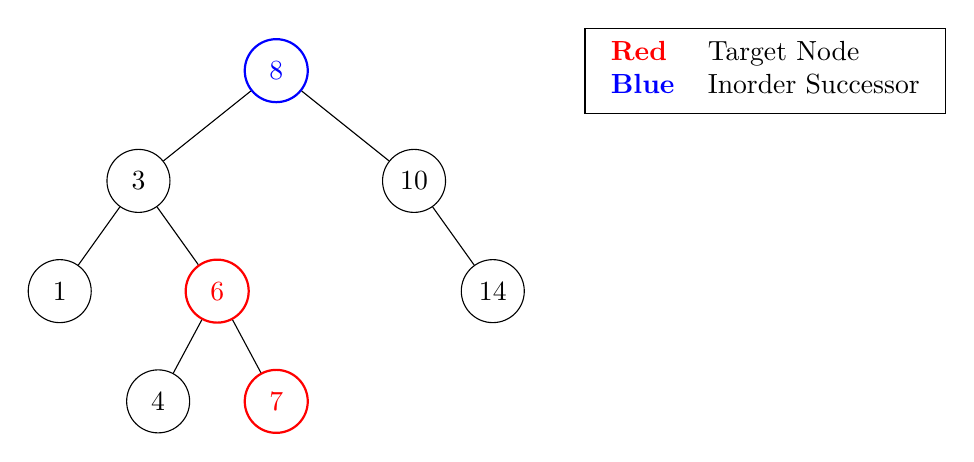
\begin{tikzpicture}[
  every node/.style={circle, draw, minimum size=0.8cm},
  level distance=1.4cm,
  level 1/.style={sibling distance=3.5cm},
  level 2/.style={sibling distance=2cm},
  level 3/.style={sibling distance=1.5cm},
  successor/.style={circle, draw, minimum size=0.8cm, thick, color=blue},
  target/.style={circle, draw, minimum size=0.8cm, thick, color=red}
]

% Tree structure
\node[successor] (n8) {8}
  child {node {3}
    child {node {1}}
    child {node[target] (n6) {6}
      child {node {4}}
      child {node[target] (n7) {7}}
    }
  }
  child {node {10}
    child[missing]
    child {node {14}}
  };

% Legend
\node[rectangle, draw, minimum width=3.2cm, minimum height=1cm, right=3.5cm of n8] (legend) {
  \begin{tabular}{ll}
  \textcolor{red}{\textbf{Red}} & Target Node \\
  \textcolor{blue}{\textbf{Blue}} & Inorder Successor
  \end{tabular}
};

\end{tikzpicture}
\end{center}

\textbf{Case 1:}  
Node \textbf{6} has a right child (7). Its inorder successor is the leftmost node in its right subtree: \textbf{7}.



\textbf{Case 2:}  
Node \textbf{7} has no right subtree. To find its inorder successor:

\begin{itemize}
  \item We move up the tree from node 7 to its parent (node 6), but since 7 is a \textbf{right child}, we continue upward.
  \item We then move from 6 to its parent (node 3), where 6 is a \textbf{right child} again, so we continue.
  \item We then move from 3 to node 8, where 3 is a \textbf{left child}.
  \item Hence, node \textbf{8} is the lowest ancestor where node 7 (through its lineage) lies in the left subtree.
\end{itemize}

Therefore, the inorder successor of node \textbf{7} is \textbf{8}.
\\


\textbf{C++ Implementation:}

\subsubsection*{Deletion Using \texttt{inorderSuccessor}}

\begin{lstlisting}[style=cppstyle]
// Full-tree inorderSuccessor version used here
BSTNode* deleteNode(BSTNode* root, int key) {
  if (!root) return nullptr;

  if (key < root->key)
    root->left = deleteNode(root->left, key);
  else if (key > root->key)
    root->right = deleteNode(root->right, key);
  else {
    // Case 1 and 2: Node with 0 or 1 child
    if (!root->left) {
      BSTNode* temp = root->right;
      delete root;
      return temp;
    } else if (!root->right) {
      BSTNode* temp = root->left;
      delete root;
      return temp;
    }

    // Case 3: Node with 2 children
    BSTNode* succ = inorderSuccessor(root, root); // full-tree root and current node
    root->key = succ->key;
    root->right = deleteNode(root->right, succ->key);
  }
  return root;
}
\end{lstlisting}




\subsubsection*{Deletion Function in C++}

\begin{lstlisting}[style=cppstyle]
BSTNode* deleteNode(BSTNode* root, int key) {
  if (!root) return nullptr;

  if (key < root->key)
    root->left = deleteNode(root->left, key);
  else if (key > root->key)
    root->right = deleteNode(root->right, key);
  else {
    // Case 1 and 2: Node with 0 or 1 child
    if (!root->left) {
      BSTNode* temp = root->right;
      delete root;
      return temp;
    }
    else if (!root->right) {
      BSTNode* temp = root->left;
      delete root;
      return temp;
    }

    // Case 3: Node with 2 children
    BSTNode* succ = findMin(root->right);
    root->key = succ->key;
    root->right = deleteNode(root->right, succ->key);
  }
  return root;
}
\end{lstlisting}

\textbf{Note:} The deletion algorithm maintains the BST invariant by rearranging nodes appropriately. If balance is not preserved, performance can degrade to $\mathcal{O}(n)$.

\subsection{Degenerate Cases and Balancing}

A poorly structured BST can degrade to a linked list, resulting in $\mathcal{O}(n)$ time operations. To prevent this:

\begin{itemize}
  \item Use self-balancing trees like AVL or Red-Black Trees
  \item Randomize insertions or rebalance periodically
\end{itemize}

Balanced BSTs ensure height $\mathcal{O}(\log n)$, which guarantees logarithmic performance for search-related operations.

\section{Tree Rotations}

Tree rotations are fundamental operations used in self-balancing binary search trees (e.g., AVL and Red-Black Trees) to restore height balance after insertions or deletions. A rotation is a local restructuring operation that preserves the BST ordering.

\subsection{Right Rotation (\texttt{rotateRight})}

Right rotation is applied at a node $y$ with a left child $x$ to reduce the height of the left subtree.

\textbf{Before:}
\[
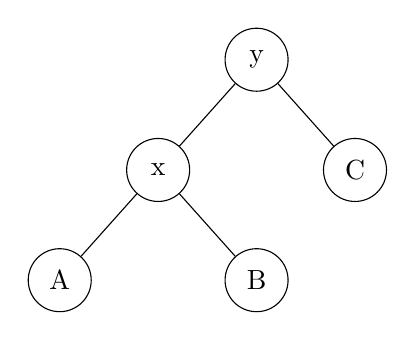
\begin{tikzpicture}[
  every node/.style={circle, draw, minimum size=0.8cm},
  level distance=1.4cm,
  level 1/.style={sibling distance=2.5cm}
]
\node (y) {y}
  child {node (x) {x}
    child {node {A}}
    child {node {B}}
  }
  child {node {C}};
\end{tikzpicture}
\]

\textbf{After \texttt{rotateRight(y)}:}
\[
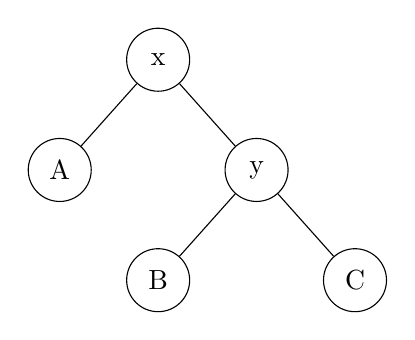
\begin{tikzpicture}[
  every node/.style={circle, draw, minimum size=0.8cm},
  level distance=1.4cm,
  level 1/.style={sibling distance=2.5cm}
]
\node (x) {x}
  child {node {A}}
  child {node (y) {y}
    child {node {B}}
    child {node {C}}
  };
\end{tikzpicture}
\]

\subsection{Left Rotation (\texttt{rotateLeft})}

Left rotation is applied at a node $x$ with a right child $y$ to reduce the height of the right subtree.

\textbf{Before:}
\[
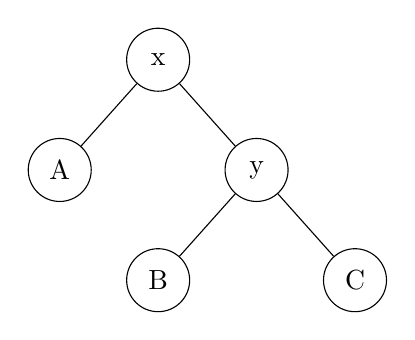
\begin{tikzpicture}[
  every node/.style={circle, draw, minimum size=0.8cm},
  level distance=1.4cm,
  level 1/.style={sibling distance=2.5cm}
]
\node (x) {x}
  child {node {A}}
  child {node (y) {y}
    child {node {B}}
    child {node {C}}
  };
\end{tikzpicture}
\]

\textbf{After \texttt{rotateLeft(x)}:}
\[
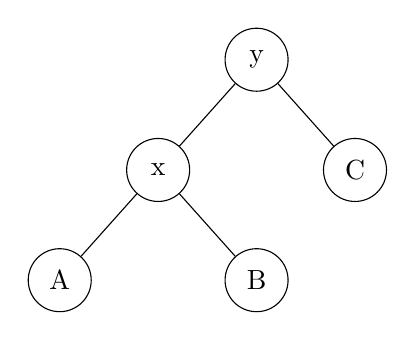
\begin{tikzpicture}[
  every node/.style={circle, draw, minimum size=0.8cm},
  level distance=1.4cm,
  level 1/.style={sibling distance=2.5cm}
]
\node (y) {y}
  child {node (x) {x}
    child {node {A}}
    child {node {B}}
  }
  child {node {C}};
\end{tikzpicture}
\]

\subsection{Preserving the BST Property During Rotations}

Tree rotations maintain the binary search tree property:
\[
\texttt{left subtree} < \texttt{node} < \texttt{right subtree}
\]

Consider the right rotation at node $y$ (where $x$ is its left child):

\textbf{Before rotation:}
\begin{itemize}
  \item Subtree A: All keys $<$ x.key
  \item Subtree B: x.key $<$ keys $<$ y.key
  \item Subtree C: All keys $>$ y.key
\end{itemize}

\textbf{Right Rotation:}

\[
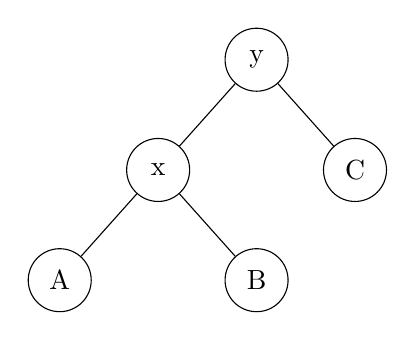
\begin{tikzpicture}[
  every node/.style={circle, draw, minimum size=0.8cm},
  level distance=1.4cm,
  level 1/.style={sibling distance=2.5cm}
]
\node (y) {y}
  child {node (x) {x}
    child {node {A}}
    child {node {B}}
  }
  child {node {C}};
\end{tikzpicture}
\quad
\Rightarrow
\quad
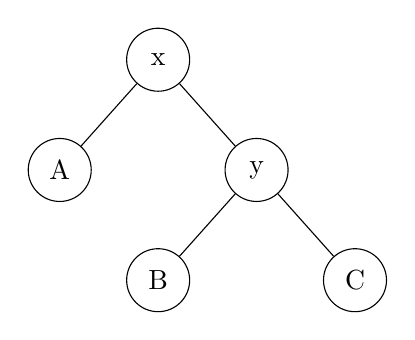
\begin{tikzpicture}[
  every node/.style={circle, draw, minimum size=0.8cm},
  level distance=1.4cm,
  level 1/.style={sibling distance=2.5cm}
]
\node (x) {x}
  child {node {A}}
  child {node (y) {y}
    child {node {B}}
    child {node {C}}
  };
\end{tikzpicture}
\]

\textbf{After rotation:}
\begin{itemize}
  \item Subtree A remains in the left of x
  \item Subtree B becomes left of y, and since B's keys were $>$ x.key and $<$ y.key, they remain valid
  \item Subtree C remains to the right of y
\end{itemize}

All relative key orderings are preserved, satisfying:
\[
\texttt{A} < x < \texttt{B} < y < \texttt{C}
\]


Both left and right rotations preserve in-order traversal and relative ordering of keys. Hence, the BST property remains intact after any single rotation.

\section{Practice problem}
Leetcode Problem 108: \textit{Convert Sorted Array to Binary Search Tree}

\url{https://leetcode.com/problems/convert-sorted-array-to-binary-search-tree/description/}

\end{document}